\documentclass[11pt]{article}
\usepackage{fullpage,amsmath,mathtools, algorithm2e, forest}
\usepackage[mathletters]{ucs}
\usepackage{hyperref}
\usepackage[utf8x]{inputenc}
\usepackage{graphicx}
\usepackage{listings}
\usepackage{courier}

\lstset{basicstyle=\footnotesize\ttfamily,breaklines=true}
\lstset{frame=single}

\graphicspath{ {./images/} }
\title{COMP4107 - Assignment 1}
\author{Student Name: Yunkai Wang\\
\text{Student Number: 100968473}\\\\
Student Name: Jules Kuehn\\
\text{Student Number: 100661464}}
\date{Fall 2018}
\begin{document}
\maketitle
\begin{enumerate}

\item Question 1\newline
Implementation for question 1 can be found in q1.py. The result is\\
\lstinputlisting{python_output/q1.out}
Notice that the matrices $U, V$ are different with the matrices in the slide, however, in order to generate the same result, we have to take the transpose of the original matrix, which is not something that we decided to go with since I don't think we are allowed to do that. The closest user in 2D is Alicia, and the closest user in 4D is Mary.

\item Question 2\newline
Implementation for question 2 can be found in q2.py. The result is\\
\lstinputlisting{python_output/q2.out}

\item Question 3\newline
Implementation for question 3 can be found in q3.py. The best rank(2) matrix takes the first 2 values since s is sorted descending. The result is very good.\\
\lstinputlisting{python_output/q3.out}

\item Question 4\newline
Implementation for question 4 can be found in q4.py. The only learning rate that will work is when $ε = 0.01$, which will lead to the correct result with $\approx 420$ iterations. The other ones won't work as we are descending too quickly, and therefore we will miss the correct answer and failed to come back. It "bounces around" the correct result, while the norm continues to increase. We set the program to stop once the norm of the vector is greater than $100000$, which is obviously too big and therefore it's impossible to get the result.
\lstinputlisting{python_output/q4.out}

\item Question 5\newline
The implementation for q5 can be found in q5.py. $A = \begin{bmatrix} 3 & 2 & -1 & 4 \\ 1 & 0 & 2 & 3 \\ -2 & -2 & 3 & 3\end{bmatrix}$. It's clear that the rows of $A$ are not linearly independent. To see this, we reduce $A$ to its RREF form and we will get $A = \begin{bmatrix} 1 & 0 & 2 & 3 \\ 0 & 1 & -7/2 & -5/2 \\ 0 & 0 & 0 & 0\end{bmatrix}$, rank of rows of $A$ equals to $2$. The columns of $A$ are not linearly independent either. Since as we reduce $A^T$ to RREF form, we will get $A = \begin{bmatrix} 1 &0 & -1 \\ 0 & 1 & 1 \\ 0 & 0 & 0 \\ 0 & 0 & 0\end{bmatrix}$, clearly that rank of the columns of $A$ equal to $2$, so the columns are not linearly independent. The inverse of $A$ cannot be calculated as $A$ is not a square matrix, and the rows and columns of $A$ are not linearly independent.\\
\lstinputlisting{python_output/q5.out}

\item Question 6\newline
Implementation for question 6 can be found in q6.py. The implementation correctly replicated the results of the paper, for the entire set of 10000.\newline
Also included are plots from a random sample of 1000, followed by 3 random samples of 100.\newline
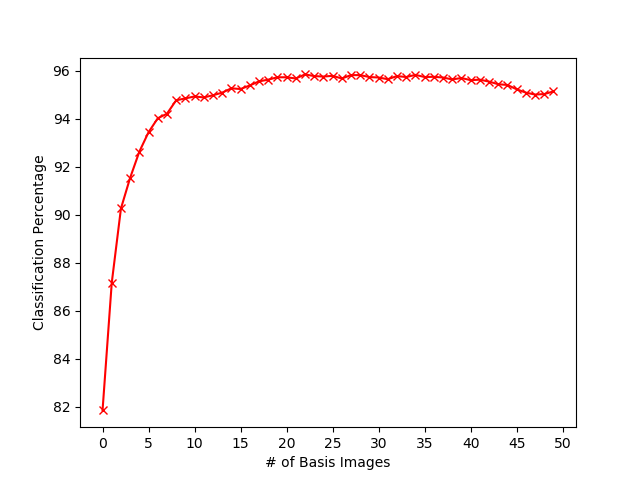
\includegraphics[width=0.7\columnwidth]{q6-graphEntireSet10000}\newline
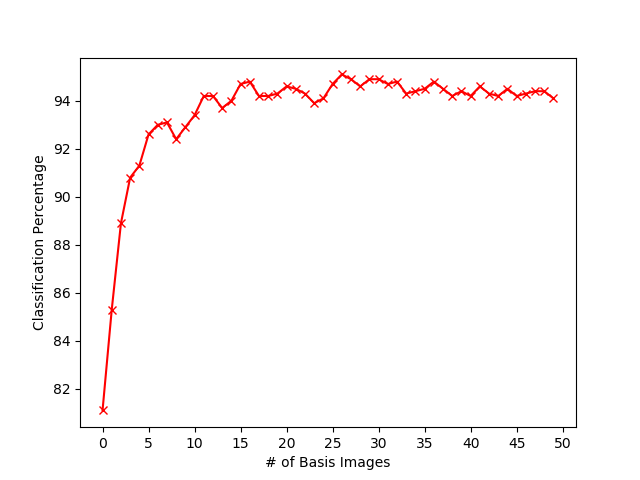
\includegraphics[width=0.7\columnwidth]{q6-graphRandomSample1000}\newline
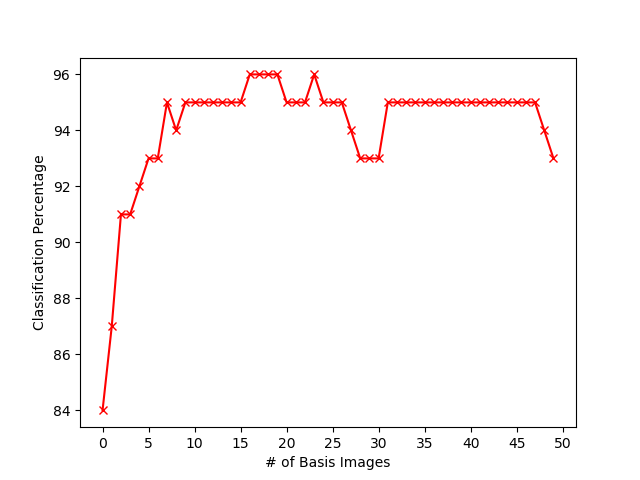
\includegraphics[width=0.7\columnwidth]{q6-graphRandomSample100-1}\newline
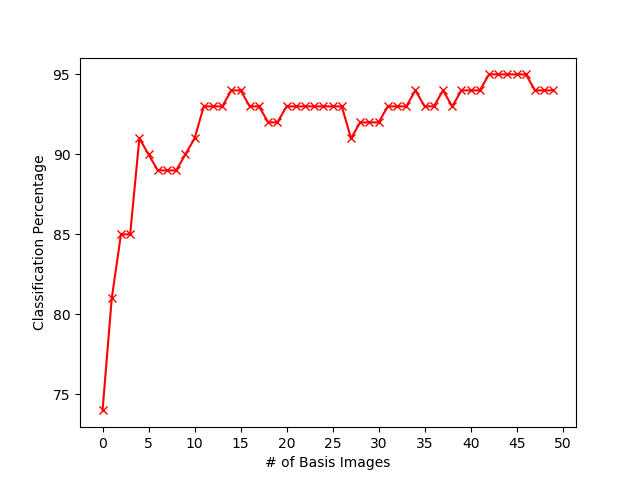
\includegraphics[width=0.7\columnwidth]{q6-graphRandomSample100-2}\newline
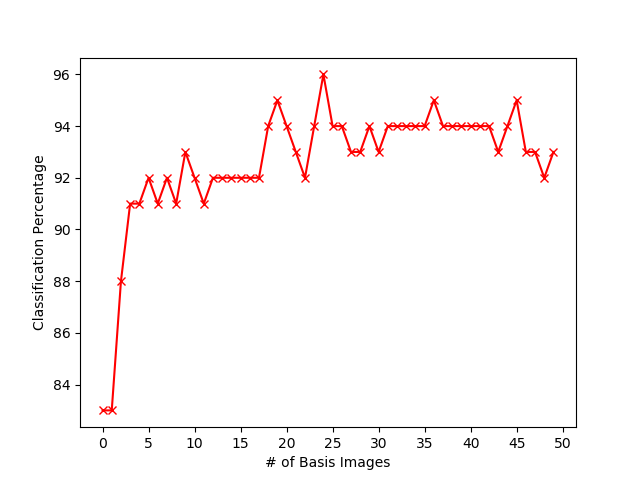
\includegraphics[width=0.7\columnwidth]{q6-graphRandomSample100-3}

\item Question 7\newline
Implementation for question 7 can be found in q7.py. To accomplish question 7, we read another paper online which can be found at \href{https://drive.google.com/file/d/0BylQe2cRVWE_RmZoUTJYSGZNaXM/view}{here}. We used the filling-in of missing data, and normalization method from this paper. We used the folding in method mentioned in the paper referenced by the assignment, producing the following results.

\lstinputlisting{python_output/q7.out}
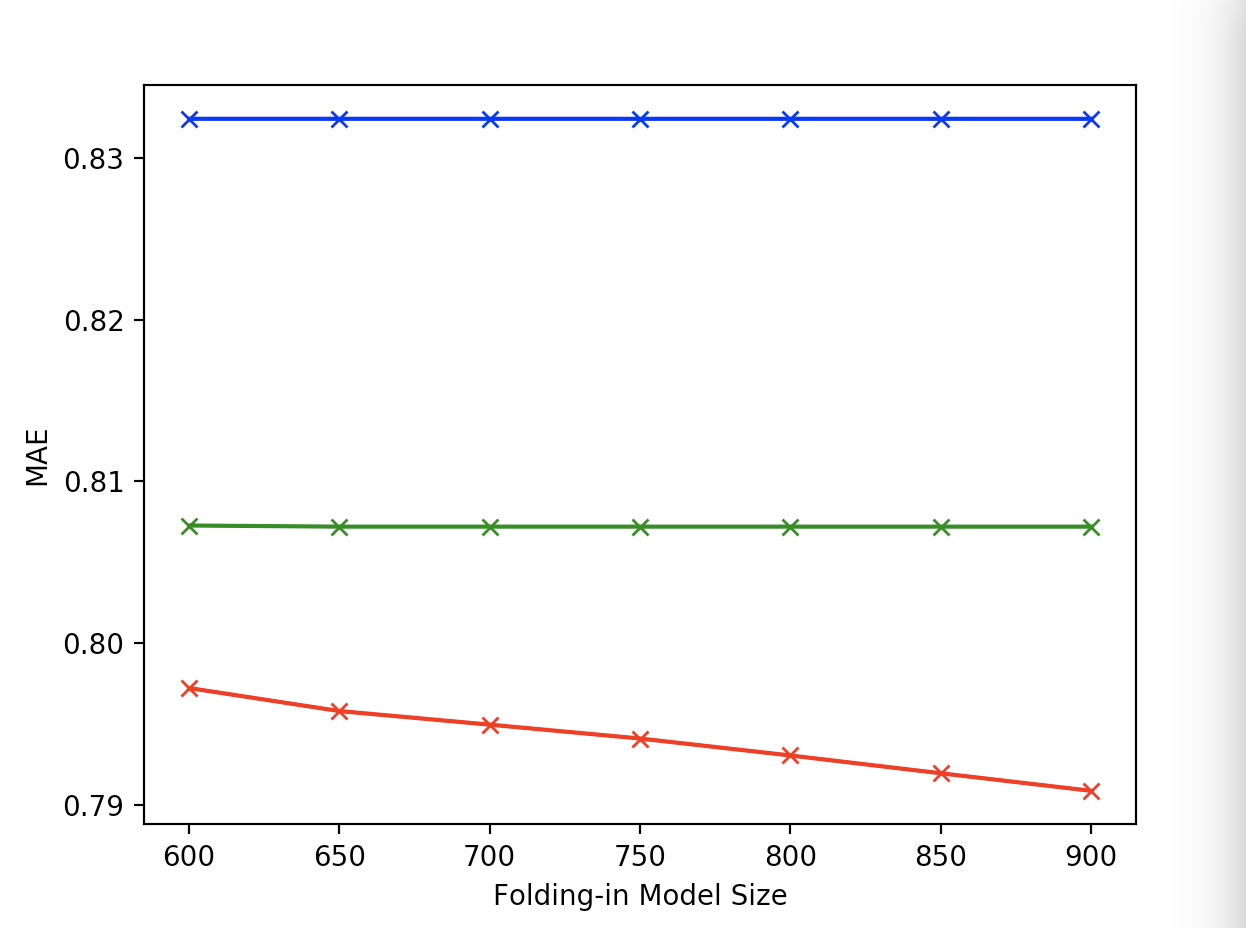
\includegraphics[width=0.7\columnwidth]{q7_result1}\newline
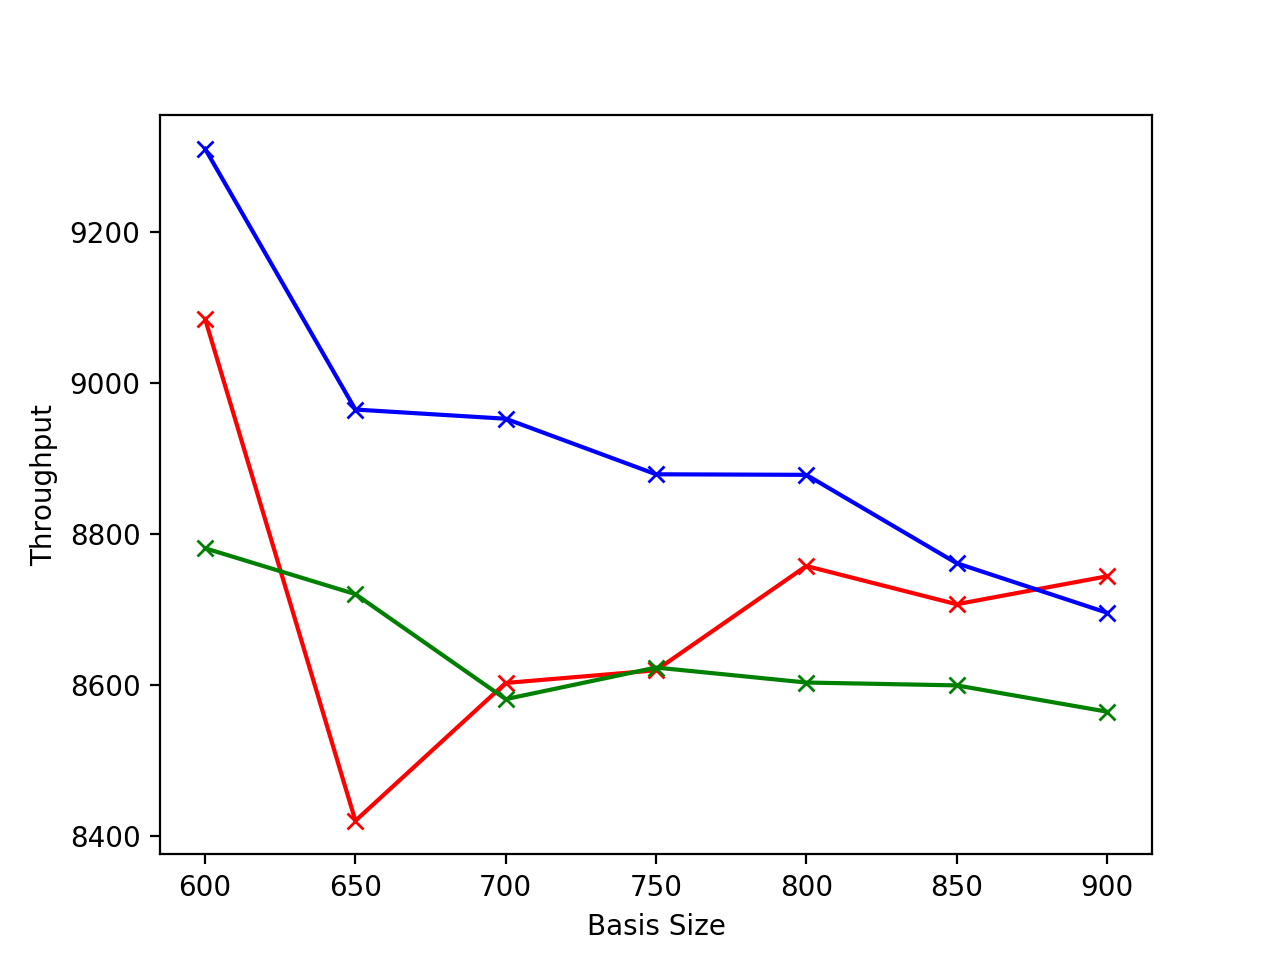
\includegraphics[width=0.7\columnwidth]{q7_result3}

\end{enumerate}
\end{document}